\documentclass[../report.tex]{subfiles}
\graphicspath{{\subfix{../image/}}}

\begin{document}
\maketitle

\section*{Introduction}

One of the main focuses of this third semester project is the analog components. Electronics bring the software and the mechanical part together. 
The software needs feedback from the analog world. It needs to know how heavy the load is and
whether there is an obstacle in front. All these tasks necessary to guarantee safe operations.

\quad
The tasks include the following:

\begin{itemize}
    \item Interfacing the analog load cells
    \item Power Supply
    \item Motor Drivers
\end{itemize}

\begin{figure}[h!]
    \centering
    \begin{subfigure}[b]{0.4\linewidth}
      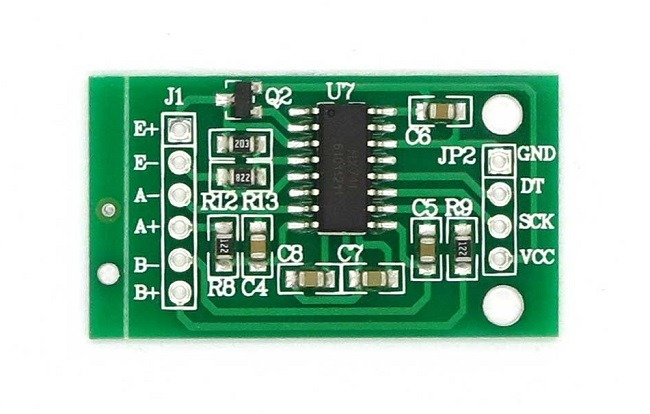
\includegraphics[width=\linewidth]{image/HX711-Weighing-Sensor-Dual-Channel-24-Bit-Precision-A-D-Module-Pressure-Sensor_1.jpg}
      \caption{HX711 Interface Module }
    \end{subfigure}
    \begin{subfigure}[b]{0.4\linewidth}
      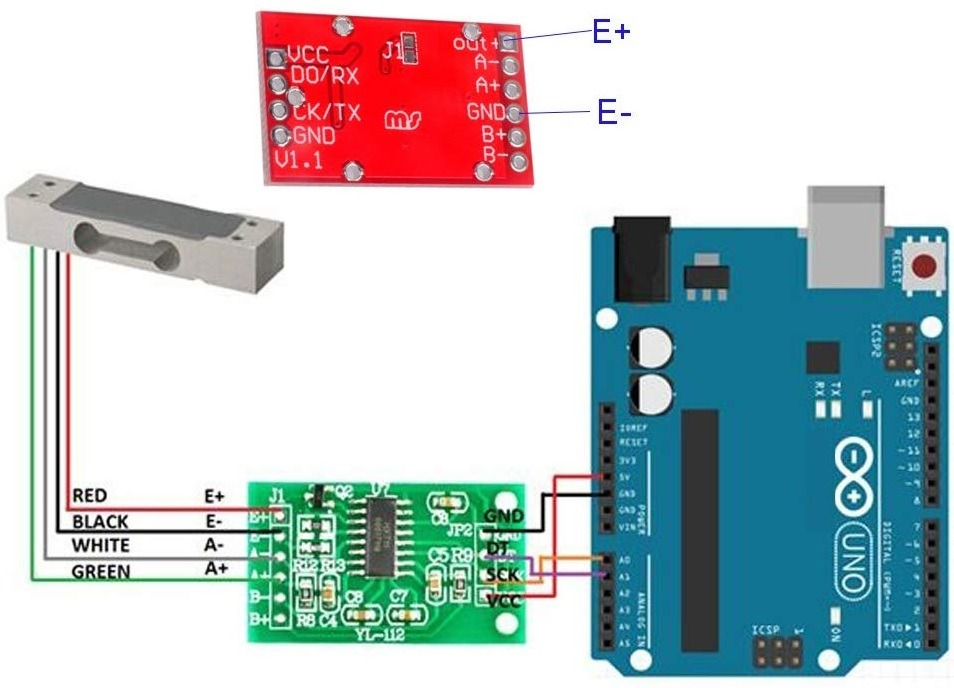
\includegraphics[width=\linewidth]{image/hx711-red.jpg}
      \caption{HX711 Interface Module and Load cell using Arduino}
    \end{subfigure}
    
    
  \end{figure}
  
\end{document}